\section{Introduction}
\label{sec:intro}

% ~\cite{dblp_hotos}, ~\cite{Rashid:1989}, ~\cite{Welch:1989}, ~\cite{Satya:1989}, ~\cite{cs523}


The fundamental basis for various services today lies in the effective provision of robust distributed systems. The assurance of resilience within such systems remains a critical area of investigation, mainly due to the systems' vulnerability to a range of distinct failure patterns.
The research by \textit{Bronson et al.}\cite{mtsb_hotos} characterizes metastable failures as a subset of failures that trap a system in a compromised state with low throughput, even after the original triggering event has been resolved. These failures constitute a distinctive category within the spectrum of failures, distinguished by their emergent nature and the absence of a clear and direct link between the initial event and the underlying cause that sustains the failure.

The life cycle of a system susceptible to this category of failures consists of three distinct states: the stable state, the vulnerable state, and the metastable state. All systems start in the stable state and gradually move to the vulnerable state as the load increases. Once the system enters the vulnerable state, it remains healthy and can persist in this state for a long duration. However, when a triggering event occurs, it becomes stuck in the metastable state. Interestingly, most production systems prefer to operate in the vulnerable state since it offers better resource utilization.

Metastable failures can significantly reduce a system's efficiency without necessarily causing it to crash, which is why they might not be immediately noticeable. Another intriguing aspect is that overcoming metastable failures often requires drastic measures such as system reboots or load shedding, which could lead to further disruptions. Given the nature of this failure pattern, it becomes imperative to detect it proactively before it occurs. 
\begin{figure}[h]
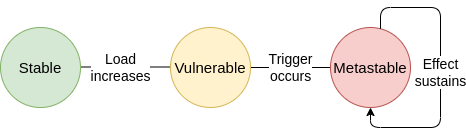
\includegraphics[width=0.45\textwidth]{images/mtsb.drawio.png}
\caption{Life cycle of a system vulnerable to metastable failures.}s
\end{figure}

In view of the pressing need for solutions in this domain, our paper seeks to take the initial strides towards the formidable objective of facilitating metastability detection in diverse distributed systems. The ultimate aim is to create a tool capable of assessing a given distributed system and gauging its susceptibility to metastability. This tool could also potentially propose strategies to mitigate this vulnerability or give the conditions which will lead to the metastable state.

Despite the various observed cases, they all share a common trait: a decrease in goodput even after the load returns to normal. We emphasize this pivotal juncture and undertake two strategies to identify the conditions that lead to this point:
\begin{itemize}
    \item formally model the system based on the domain knowledge
    \item derive a model of the system based on the runtime behavior.            
\end{itemize}
We assess the feasibility of both approaches, along with their respective accuracies.

We opt for Petri nets as our modeling tool due to their usage in recent research work. Additionally, Petri nets possess the capability to represent concurrent events and resource utilization effectively. However, as the paper demonstrates, system modeling is by no means a straightforward task, demanding a substantial investment of effort, even for a synthetic example. Moreover, a profound comprehension of the system's inherent intricacies is essential for its accurate formal modeling; otherwise, the model may yield misleading outcomes and inaccurately report conditions. Ensuring the model's accuracy also presents a challenging and complex problem.
